\documentclass[twoside,numberorder]{csbachelor}
%==============================================================
%==============================================================

\usepackage{url}
\usepackage{subfigure}

%一些全局工具的定义
\DeclareMathOperator*{\argmin}{arg\,min}
\DeclareMathOperator*{\argmax}{arg\,max}

%==============================================================
%==============================================================
\begin{document}
%==============================================================
%==============================================================

  %论文题目:{中文}{英文}
  \zjutitle{中文题目}%
           {english title}
  %作者:{中文姓名}{英文}{学号}
  \zjuauthor{瞿泽宁}{Qu Zening}{3080102955}
  %指导教师:{导师中文名}{导师英文名}
  \zjumentor{彭群生}{Peng Qunsheng}
  %个人信息:{年级}{专业名称}
  \zjuinfo{2008级}{计算机科学与技术}
  %学院信息:{学院中文}{学院英文}
  \zjucollege{计算机科学与技术学院}{College of Computer Science and Technology}
  %日期:{Submitted Date}
  \zjudate{}

%==============================================================

  %封面
  %%============================================================
%% 中文封面

\thispagestyle{empty}

\vspace{5mm}

\begin{center}
   
\includegraphics[width=108mm]{images/zjdx}
\end{center}

\centerline{\songti\xiaoyi\textbf{本科生毕业论文}}
\centerline{\songti\xiaoyi\textbf{开题报告}}
\vspace{4mm}

\begin{center}
  
\includegraphics[width=35mm]{images/standxb}
\end{center}

\vspace{32mm}

\begin{tabbing}
               \hspace{30mm} \= \songti\sihao 学生姓名: \= \underline{\makebox[6cm]{\sihao\zjuauthornamec}} \\[2mm]
              \> \songti\sihao 学生学号: \> \underline{\makebox[6cm]{\sihao\zjuauthorid}} \\[2mm]
              \> \songti\sihao 指导教师: \> \underline{\makebox[6cm]{\sihao\zjumentorc}} \\[2mm]
              \> \songti\sihao 专\hspace{10mm}业: \> \underline{\makebox[6cm]{\sihao\zjugrade\hspace{3mm}\zjumajor}} \\[2mm]
              \> \songti\sihao 学\hspace{10mm}院: \> \underline{\makebox[6cm]{\sihao\zjucollegec}}
\end{tabbing}


%%============================================================
% empty page for two-page print
\ifthenelse{\equal{\zjuside}{T}}{%
  \newpage\mbox{}%
  \thispagestyle{empty}}{}

  %诚信承诺书
  %% mentorassign

\newpage
\thispagestyle{empty}

\begin{tabbing}
\hspace{5mm}\songti\sihao 一、题目:\underline{\makebox[12cm]{}}
\\ \\
\hspace{5mm}\songti\sihao 二、指导教师对开题报告、外文翻译和文献综述的具体要求:
\end{tabbing}

\vspace{140mm}

\begin{tabbing}
\hspace{80mm}\songti\xiaosi 指导教师(签名):
\\ \hspace{90mm} \songti\xiaosi 年 \hspace{5mm} \songti\xiaosi 月 \hspace{5mm} \songti\xiaosi 日
\end{tabbing}

\ifthenelse{\equal{\zjuside}{T}}{%
  \newpage\mbox{}%
  \thispagestyle{empty}}{}

  %考核
  %考核
\thispagestyle{empty}
\begin{center}
\stfangsong\sanhao 毕业论文开题报告、外文翻译和文献综述考核
\end{center}
\songti\sihao 导师对开题报告、外文翻译和文献综述评语及成绩评定:
\vspace{4cm}

{
\hspace{3cm} \songti\xiaosi
\begin{tabular}{|c|c|c|c|}
    \hline
    成绩比例 & \parbox[t]{4em}{开题报告\\[-3.5em]占(20\%)} &
               \parbox[t]{4em}{中期报告\\[-3.5em]占(10\%)} &
               \parbox[t]{4em}{外文翻译\\[-3.5em]占(10\%)} \\

    \hline
    分值   & & &  \\
    \hline
\end{tabular}
}
\begin{flushright}
    导师签字\;\underline{\hspace{4em}}\\
    年 \quad 月 \quad 日
\end{flushright}
\vspace{-1cm}
{\songti\sihao 答辩小组对开题报告、外文翻译和文献综述评语及成绩评定:}
\vspace{4cm}

{
\hspace{3cm} \songti\xiaosi
\begin{tabular}{|c|c|c|c|}
    \hline
    成绩比例 & \parbox[t]{4em}{开题报告\\[-3.5em]占(20\%)} &
               \parbox[t]{4em}{文献综述\\[-3.5em]占(10\%)} &
               \parbox[t]{4em}{外文翻译\\[-3.5em]占(10\%)} \\

    \hline
    分值   & & &  \\
    \hline
\end{tabular}
}
\begin{flushright}
    答辩小组负责人(签名)\;\underline{\hspace{4em}}\\
    年 \quad 月 \quad 日
\end{flushright}



%==============================================================
%这部分不需要自己修改。

  %目次页
  \tableofcontents
  \thispagestyle{empty}
  \chaptermark{目录}
  %\addcontentsline{toc}{chapter}{目录}

  \mainmatter

%==============================================================

  \chapter{本科毕业论文开题报告}
%字数要求3500字以上
%课题意义、背景及可行性分析、调研报告、研究方案、实施计划、预期结果等
\section{课题背景}

\section{目标和内容}

\section{可行性分析}

\section{研究方案和关键技术考虑}

\section{预期研究结果}

\section{进度计划} 

  \chapter{本科毕业论文文献综述}




  \chapter{本科毕业论文外文翻译}
%字数要求3000字

\heiti
摘要

\songti
当今世界,网络已被内容(content)的散布和获取所主导,而网络技术却仍然只言主机间连接而不及其它。%其它指物,其他指人。
为获取网络内容和服务,须要建立起一个从网络用户所关心的(内容)到网络中的位置的映射。%需要主观且物质,须要客观且抽象
我们提出内容为心网络(Content-Centric Networking~简称~CCN)。它以内容为原语——把网络位置与网络身份、安全和访问分离开来,用名字访问内容。我们从IP推演出适用于命名内容的路由算法。使用这些算法,我们可以使网络的可扩展性、安全性和性能同时达到要求。我们实现了我们的体系结构的基本框架,用安全文件下载和VoIP电话两个例子演示了网络的性能和可恢复性。

\heiti
类别和学科描述符

\songti
C.2.1~[计算机系统组织]:网络结构与设计;~C.2.2~[计算机系统组织]:网络协议

\heiti
通用术语

\songti
设计,实验,性能,安全



%===========================%
\section{引言}
今天的互联网背后的工程原理和体系结构创建于二十世纪六、七十年代。网络致力于解决的问题是资源共享的问题——远程使用如读卡器、高速磁带机甚至超级计算机等珍贵资源。这样产生的通信模型是一个仅仅存在于两台机器之间的对话模型,一台机器希望使用资源,另一台机器为前者提供资源。因此IP包含有两个地址,一个是发送方的,一个是目的地机器的,并且互联网上几乎所有的通信都包含TCP对话。

自包交换网络被创造的50年来,计算机及其附件已经成为廉价、普适的商品。互联网的连通性和低价的存储成本使得对海量新内容的访问成为可能——仅2008年就有500艾字节的信息被生产出来~[13]。人们在意的是互联网所承载的东西,而通信仍然在谈论这些东西都在哪些地方。

我们看到这个矛盾给用户带来三方面的(负面)影响。

\begin{description}
\item[可用性]为快速、可靠地访问内容,不仅须要如~CDN~和~P2P~网络这样繁冗的,预先设计好的,面向应用软件的机制,而且还会大幅增加带宽成本。
\item[安全性]对内容的信任这一概念被偷换为不那么可信的对物理位置和网络连接的的信任。
\item[位置迁就]建立从内容到物理位置的映射使网络服务的配置和实现工作都变得复杂。
\end{description}

解决这些问题的直接办法就是把网络中的“在哪里”(where)替换为“是什么”(what)。主机到主机对话是为了解决六十年代的问题而提出的抽象模型。对于如今的通信问题,我们认为命名数据(named data)是比命名主机(named hosts)更好的模型。我们提出内容为心网络(CCN),一个建立于命名数据之上的网络架构。即使是在CCN的最底层,我们也没有位置的概念——一个CCN包的“地址”是一个内容的名字,而不是这个内容的位置。不过,我们也保留了当年使~TCP/IP~简单、稳健、可扩展的那些设计决策。

\begin{figure}
  \centering
  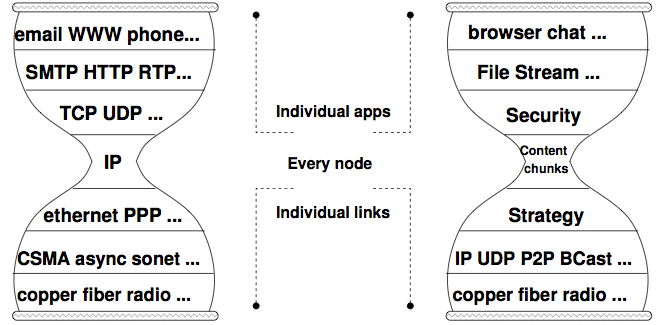
\includegraphics[width=0.7\textwidth]{images/narrow_waist}
  \caption{CCN~把网络协议栈中全局性的成分由IP换为了命名内容块} %不确定
  \label{narrow_waist}
\end{figure}

图~\ref{narrow_waist}~比较了~IP~和~CCN~协议栈。其中很多层都反映了双端约定;例如,第二层的成帧协议就反映了物理层上两端的约定,而第四层的传输协议就是一些信息生产者和消费者之间的约定。唯一一个需要全局约定的层就是第三层,即网络层。~IP~的成功在很大程度上要归功于它的网络层的简洁和它在网络第二层处提出的低要求,即:无状态,不可靠,无序,尽力交付。~CCN~的网络层(详见~\ref{sec:3})与~IP~的网络层很相似且~CCN~对第二层的要求更少,这使得它非常具有吸引力。除此之外,~CCN~可以单独成层,放置于任何一层之上,包括放置于~IP~层之上。%这一段我不是很清楚,尤其是最后一句

CCN~与~IP~有几点关键性的不同。其中两点即策略和安全已经以新层的方式在协议栈中展示了出来。由于~CCN~与第二层的关系更为简单,它可以最大限度地利用众多同时存在的网络的连通性(如以太网,~3G~,蓝牙和~802.11~等等)。~CCN~的策略层(详见~\ref{sec:3.3})为在不断变化的环境下最好地开发利用多种网络的连通性不断地做出细粒度、动态优化的选择。~CCN~确保的是内容本身的安全(详见~\ref{sec:5}),而不是内容走过的连接的安全。因此~CCN~没有许多基于主机网络的弱点,而不像~IP~网络那样深受其害。

我们在~\ref{sec:2}~至~\ref{sec:5}~中叙述了~CCN~的体系结构和运行方式。在~\ref{sec:6}~中我们评估了我们样板网络的性能。最后,在~\ref{sec:7}~和~\ref{sec:8}~中,我们讨论了相关工作并做出了结论。



%===========================%
\section{CCN~节点模型}
\label{sec:2}

\begin{figure}
  \centering
  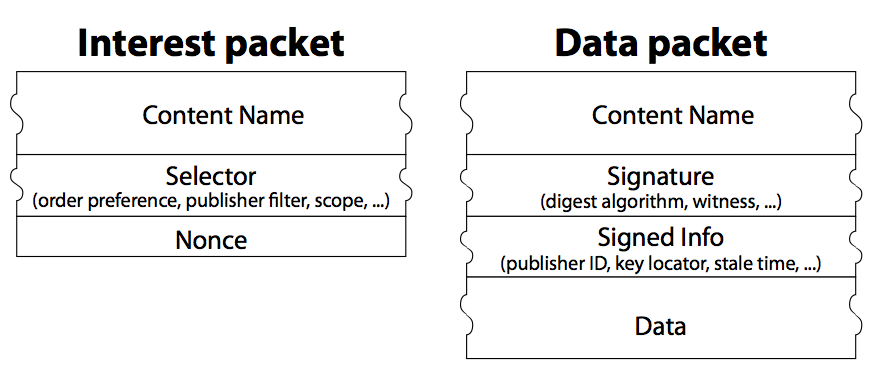
\includegraphics[width=0.7\textwidth]{images/packet_types}
  \caption{CCN~包的类型} 
  \label{packet_types}
\end{figure}

CCN~通信是由数据消费者驱动的。~CCN~包分为两类:兴趣包(Interest)和数据包(Data)(如图~\ref{packet_types})。消费者通过向所有连通之处广播自己的兴趣包来索要内容。任何一个收到兴趣包并且拥有满足该兴趣包的数据的节点都可以用一个数据包来回应该兴趣包。数据包仅为回应一个兴趣包而生,并且数据包产生之后这个收到的兴趣包就被“消费”了。
\renewcommand\baselinestretch{1} %调一下脚注行间距
\footnote{数据包和兴趣包因此是一对一的。它们保持这严格的流平衡。~TCP~中有一个类似的流平衡,即数据包和~ack~包之间的平衡。这一平衡赋予了~TCP~可扩展性和强适应性~[20]。然而与~TCP~不同的是,~CCN~模型对于多对多多点递送同样奏效(详见~\ref{sec:3.1})。}
因为兴趣包和数据包都用名字(name)来辨识内容,所以对同一个内容感兴趣的多个节点可以共享一个广播介质。其间只要使用标准的多播风暴抑制技术即可控制网络负荷~[3]。%不确定

\begin{figure}
  \centering
  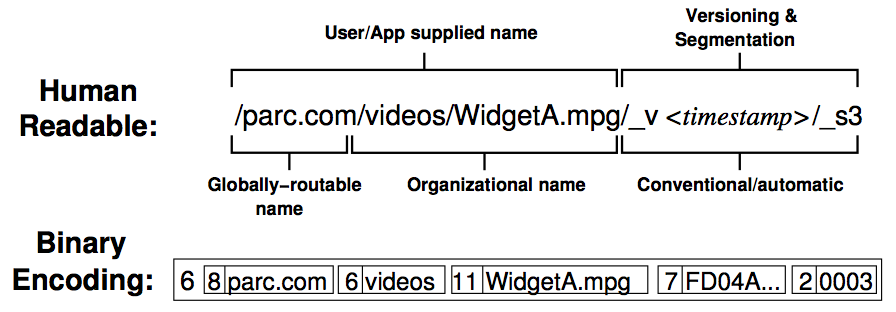
\includegraphics[width=0.7\textwidth]{images/name}
  \caption{名字示例} 
  \label{name}
\end{figure}

如果兴趣包中的内容名字(ContentName)是数据包中内容名字的前缀,那么我们称数据包“满足”了兴趣包。~CCN~名字是由若干名字部件(component)组成的不透明二元对象(如图~\ref{name})。名字一般是结构化的,因此如果前缀匹配则意味着数据包的名字是兴趣包的名字的子树(详见~\ref{sec:3.2})。~IP~使用了这种习惯来解析 <网络,子网,主机>这一层次结构。经验表明这样做既可以有效地将路由和转发状态结构化地集成,又可以支持快速查找。%极不确定
\renewcommand\baselinestretch{1} %调一下脚注行间距
\footnote{虽然~CCN~的名字是不定长的并且通常比~IP~地址要长,但是它们可以被高效地检索。一个~IP~地址的结构不是显式的,而是隐式地由节点的转发表决定的。因此,对~IP~查找使用现代~O(1)~哈希技术是十分困难的。所以~IP~查找通常使用~log(n)~的基数树检索或者并行但昂贵的~TCAMs~高端硬件。由于~CCN~的名字结构是显示的,内容名字可以很容易地被哈希,以便查找。}
这中匹配方式暗藏着这样一种可能性:内容尚未被生产出来,兴趣包就已经收到了——这使得发布者可以根据收到的数据请求实时地生产内容以回应兴趣。今天的网络中既有很多静态缓存着的数据,又有很多动态生成的数据,~CCN~灵活变化的名字机制使得它不论应对哪种数据都游刃有余。~CCN~名字还可以是上下文相关的,比如用~/ThisRoom/projector~与当前房间的投影仪交换信息,又如用~/Local/Friends~与本地(广播)环境上的任一好友交流。
\renewcommand\baselinestretch{1} %调一下脚注行间距
\footnote{这第二个例子会用到~CCN~签名机制产生的身份信息使好友们能用固定的名字约会而不是使用复杂的枚举或是探测算法。换言之,名字表示谈话的内容,而签名表示谈话者在上下文中的身份,如“本地的一个好友”。}

\begin{figure}
  \centering
  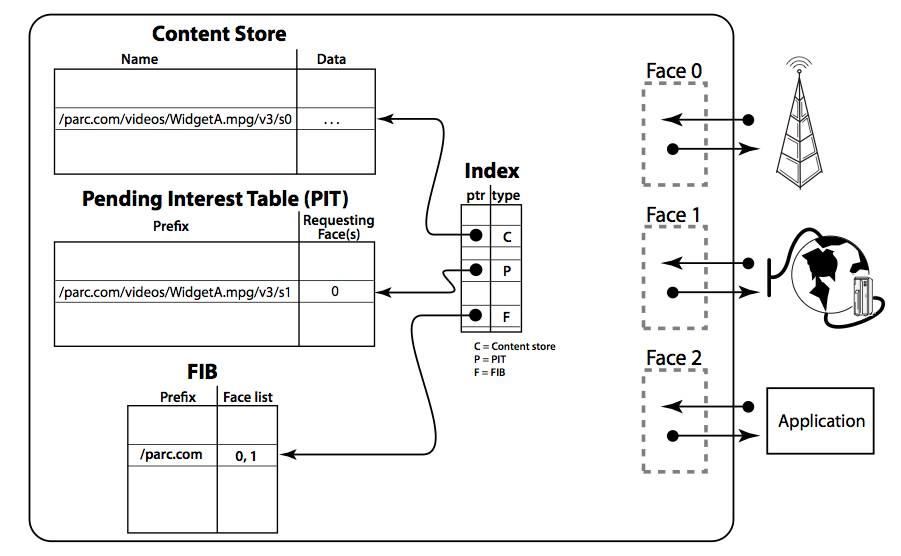
\includegraphics[width=0.7\textwidth]{images/engine}
  \caption{CCN~转发引擎模型} 
  \label{engine}
\end{figure}

CCN~节点的基本运营方式与~IP~节点非常相似:当一个包到达时,(节点)会先做一个最长名字匹配,后续操作由匹配结果而定。图~\ref{engine}~展示了~CCN~的转发引擎。它有三个主要的数据结构:~FIB(Forwarding Information Base,转发中心),CS(Content Store,内容缓存)和~PIT(Pending Interest Table,待理兴趣表)。

FIB~用于将兴趣包转发给潜在数据源。它与~IP FIB~几乎相同,只是~CCN~的FIB会为每个兴趣包维护一个出口的列表,而~IP~的~FIB~仅需要为每个收到的包维护一个转发方向。这也反映了~CCN~在转发这方面并无限制这一事实。它允许多个数据源的存在,并允许并发地请求数据。

CS~与~IP~路由器的缓存大同小异,不过它们的置换策略略有不同。由于每个~IP~包仅仅属于一个点到点对话,它被转发了以后就不再具有任何意义了。因此~IP~路由器的做法是直接抛弃已转发的包并立即循环使用自己的缓存(MRU置换)。~CCN~包是幂等的,能够自我鉴别和自我认证,因此每一个~CCN~包都有被很多用户重用的潜力(如许多主机阅读同一份电子报纸或许多用户观看同一段~Youtube~视频)。为了使多个用户分享同一内容的概率最大化(这会带来上行带宽需求最小化和下行延时最小化等诸多裨益),~CCN~会尽可能多地储存到来的数据包(LRU或LFU置换)。

PIT~记录了数据包向数据源的转发记录,这样当数据包回到路由器时就可以按照~PIT~中的记录被转回至数据申请者(们)。在~CCN~中,数据包会在它们走向潜在数据源的路上沿途撒下“面包屑”,以便匹配的数据将来沿着这些面包屑逆行,直到找到数据申请者(们)。每一个~PIT~表项就是这样一片面包屑。当一个~PIT~表项被用于转发数据包一次之后(即数据包“消费”了对应兴趣包),这个~PIT~表项就应该被抹去了。也有一些~PIT~表项一直都等不到匹配的数据包返回,这些表项最终必须因超时而被抹去(这时数据消费者如果仍然坚持想要那份数据,就有责任对那份数据重新表达兴趣)。


%===========================%
\section{传输}
\label{sec:3}
	\subsection{可靠性与流控制}
	\label{sec:3.1}
	\subsection{编号}
	\label{sec:3.2}
	\subsection{高连通性,移动性及策略}
	\label{sec:3.3}


%===========================%
\section{路由}
\label{sec:4}


%===========================%
\section{内容为心安全}
\label{sec:5}


%===========================%
\section{评估}
\label{sec:6}


%===========================%
\section{相关工作}
\label{sec:7}


%===========================%
\section{结论}
\label{sec:8}


%===========================%
\section{参考文献}
\def\tm{\leavevmode\hbox{$\rm {}^{TM}$}} %注册符 网上找的
[1] Project CCNx\tm. \url{http://www.ccnx.org}, Sep. 2009.

[2] M. Abadi. On SDSI’s Linked Local Name Spaces. \emph{Journal of Computer Security}, 6(1-2):3–21, October 1998.

[3] B. Adamson, C. Bormann, M. Handley, and J. Macker.
\emph{Multicast Negative-Acknowledgement (NACK) Building
Blocks}. IETF, November 2008. RFC 5401.

[4] W. Adjie-Winoto, E. Schwartz, H. Balakrishnan, and
J. Lilley. The Design and Implementation of an Intentional Naming System. \emph{SIGOPS Oper. Syst. Rev.}, 33(5):186–201, 1999.

[5] A. Anand, A. Gupta, A. Akella, S. Seshan, and S. Shenker. Packet Caches on Routers: The Implications of Universal Redundant Traffic Elimination. In \emph{SIGCOMM}, 2008.

[6] H. Balakrishnan, K. Lakshminarayanan, S. Ratnasamy, S. Shenker, I. Stoica, and M. Walfish. A Layered Naming Architecture for the Internet. In \emph{SIGCOMM}, 2004.

[7] M. Caesar, T. Condie, J. Kannan, K. Lakshminarayanan,
I. Stoica, and S. Shenker. ROFL: Routing on Flat Labels. In \emph{SIGCOMM}, 2006.

[8] D. Cheriton and M. Gritter. TRIAD: A New Next-Generation Internet Architecture, Jan 2000.

[9] I. Clarke, O. Sandberg, B. Wiley, and T. W. Hong. Freenet: A Distributed Anonymous Information Storage and Retrieval System. \emph{Lecture Notes in Computer Science}, 2009:46, 2001.

[10] C. M. Ellison, B. Frantz, B. Lampson, R. Rivest, B. M. Thomas, and T. Ylonen. \emph{SPKI Certificate Theory}, September 1999. RFC2693.

[11] S. Farrell and V. Cahill. \emph{Delay- and Disruption-Tolerant Networking}. Artech House Publishers, 2006.

[12] K. Fu, M. F. Kaashoek, and D. Mazières. Fast and secure distributed read-only file system. \emph{ACM Trans. Comput. Syst.}, 20(1):1–24, 2002.

[13] J. F. Gantz et al. IDC - The Expanding Digital Universe: A Forecast of Worldwide Inform ation Growth Through 2010. Technical report, March 2007.

[14] A. Gulbrandsen, P. Vixie, and L. Esibov. \emph{A DNS RR for specifying the location of services (DNS SRV)}. IETF - Network Working Group, The Internet Society, February 2000. RFC 2782.

[15] E. Guttman, C.Perkins, J. Veizades, and M. Day. \emph{Service Location Protocol}. IETF - Network Working Group, The Internet Society, June 1999. RFC 2608.

[16] IETF. RFC 2328 – OSPF Version 2.

[17] IETF. RFC 3787 – Recommendations for Interoperable IP
Networks using Intermediate System to Intermediate System (IS-IS).

[18] IETF. RFC 4971 – Intermediate System to Intermediate System (IS-IS) Extensions for Advertising Router Information.

[19] IETF. RFC 5250 – The OSPF Opaque LSA Option.

[20] V. Jacobson. Congestion Avoidance and Control. In
\emph{SIGCOMM}, 1988.

[21] V. Jacobson, R. Braden, and D. Borman. \emph{TCP Extensions for
High Performance}. IETF - Network Working Group, The
Internet Society, May 1992. RFC 1323.

[22] V. Jacobson, D. K. Smetters, N. Briggs, M. Plass, P. Stewart,
J. D. Thornton, and R. Braynard. VoCCN: Voice-over
Content-Centric Networks. In \emph{ReArch}, 2009.

[23] C. Kim, M. Caeser, and J. Rexford. Floodless in SEATTLE:
A Scalable Ethernet Architecture for Large Enterprises. In
\emph{SIGCOMM}, 2008.

[24] T. Koponen, M. Chawla, B.-G. Chun, A. Ermolinskiy, K. H.
Kim, S. Shenker, and I. Stoica. A Data-Oriented (and
Beyond) Network Architecture. In \emph{SIGCOMM}, 2007.

[25] J. Kubiatowicz et al. OceanStore: An architecture for
global-scale persistent storage. \emph{SIGPLAN Not.},
35(11):190–201, 2000.

[26] D. Mazières, M. Kaminsky, M. F. Kaashoek, and E. Witchel.
Separating Key Management from File System Security. In
\emph{SOSP}, 1999.

[27] R. C. Merkle. \emph{Secrecy, authentication, and public key
systems}. PhD thesis, 1979.

[28] R. Moskowitz and P. Nikander. \emph{Host Identity Protocol
Architecture}. IETF - Network Working Group, May 2006.
RFC 4423.

[29] B. Ohlman et al. First NetInf architecture description, April
2009. \url{http://www.4ward-project.eu/index.
php?s=file_download&id=39}.

[30] E. Osterweil, D. Massey, B. Tsendjav, B. Zhang, and
L. Zhang. Security Through Publicity. In \emph{HOTSEC}, 2006.

[31] B. C. Popescu, M. van Steen, B. Crispo, A. S. Tanenbaum,
J. Sacha, and I. Kuz. Securely replicated web documents. In
\emph{IPDPS}, 2005.

[32] R. L. Rivest and B. Lampson. SDSI - A Simple Distributed
Security Infrastructure. Technical report, MIT, 1996.

[33] M. Särelä, T. Rinta-aho, and S. Tarkoma. RTFM:
Publish/Subscribe Internetworking Architecture. In
\emph{ICT-MobileSummit}, 2008.

[34] D. K. Smetters and V. Jacobson. Securing network content,
October 2009. PARC Technical Report.

[35] I. Stoica, D. Adkins, S. Zhuang, S. Shenker, and S. Surana.
Internet Indirection Infrastructure. In \emph{SIGCOMM}, 2002.

[36] I. Stoica, R. Morris, D. Karger, F. Kaashoek, and
H. Balakrishnan. Chord: A Scalable Peer-To-Peer Lookup
Service for Internet Applications. In \emph{SIGCOMM}, 2001.

[37] D. Wendlandt, D. Andersen, and A. Perrig. Perspectives: Improving SSH-style host authentication with multi-path
probing. In \emph{USENIX}, 2008.

%==============================================================
%这也是个不需要自己修改的部分。

  \backmatter %结束章节自动编号

%==============================================================
\end{document}
